\documentclass[handout]{beamer}
\usepackage[utf8]{inputenc}
\usepackage{ stmaryrd }
\usepackage{tikz}

\usepackage{physics}
\usepackage{hyperref}
\usepackage{amsmath}
\usepackage{amsthm}
\usepackage{amssymb}
\usetheme{Madrid}
% \mode<presentation>{}
\usecolortheme{default}
\usepackage{mathtools}
\DeclarePairedDelimiter\ceil{\lceil}{\rceil}
\DeclarePairedDelimiter\floor{\lfloor}{\rfloor}
\newcommand{\cosec}{\operatorname{cosec}}

%------------------------------------------------------------
%This block of code defines the information to appear in the
%Title page
\title[MA109 Calculus-I] %optional
{MA109 Calculus-I}

\subtitle{D4-T6 Tutorial 5}

\author[Adish Shah] % (optional)
{Adish Shah}



\date[4th January 2022] % (optional)
{4th January 2022}



%End of title page configuration block
%------------------------------------------------------------



%------------------------------------------------------------
%The next block of commands puts the table of contents at the 
%beginning of each section and highlights the current section:

\AtBeginSection[]
{
  \begin{frame}
    \frametitle{Table of Contents}
    \tableofcontents[currentsection]
  \end{frame}
}
%------------------------------------------------------------


\begin{document}

%The next statement creates the title page.
\frame{\titlepage}

% \begin{frame}
% 	\frametitle{{Fundamental Theorem of Calculus : Part 1}}
% 	\begin{theorem}[Fundamental Theorem of Calculus : Part 1]
% 		Let $f$ be integrable on $[a, b]$. For $x \in [a,b]$,define\\
% 		\[F(x) := \int_{a}^{b}f(t)dt\] 
% 	Then $F$ is continuous on $[a,b]$. Morover, if $f$ is continuous at $c \in [a,b]$,
% 	then $F$ is differentiable at $c$, and $F'(c) = f(c)$
% 	\end{theorem}

% \end{frame}
% \begin{frame}
% 	\frametitle{{Fundamental Theorem of Calculus : Part 2}}
% 	\begin{theorem}[Fundamental Theorem of Calculus : Part 2]
% 		Let $f:[a, b] \to \mathbb{R}$ be a differentiable function such that\\
% 		$f'$ is integrable on $[a, b],$. Then\\
% 		\[\int_{a}^{b}f'(x)dx = f(b)-f(a)\]
% 	\end{theorem}
% \end{frame}

%---------------------------------------------------------
\begin{frame}
	\frametitle{1) (i)}
	Writing $y$ in terms of $x$ gives us $y = 1 - 2\sqrt{x} + x.$\\
	The desired area is $$\displaystyle\int_{0}^{1} y dx = \int_{0}^{1} (1 - 2\sqrt{x} + x) dx = \left.\left(x - 2\cdot\frac{2}{3}x^{3/2} + \frac{1}{2}x^2\right)\right|_{0}^{1} = 1 - \frac{4}{3} + \dfrac{1}{2} = \frac{1}{6}. $$\\~\\
\end{frame}


%Changing visivility of the text
\begin{frame}
	\frametitle{2)}
    It is easy to see that the curves $y = f(x)$ and $y = g(x)$ intersect at $(0, 0)$ and $(1-a, a-a^2).$\\
	Let us assume that $a < 1$ and find the area $A.$
	\[A = \int_{0}^{1-a} (x - x^2 - ax) dx = \frac{(1-a)^3}{6}.\]
	As $A = 4.5,$ we get that $(1 - a)^3 = 27.$ Thus, we have it that $a = -2.$\\
	Now, if we assume that $a > 1,$ we get that $A = \frac{(a-1)^3}{6} = 4.5$ which gives us that $a = 4.$
\end{frame}

\begin{frame}
	\frametitle{3)}
	Solving for the intersection point of the two curves gives us
	\[6a\cos\theta = 2a(1+\cos\theta) \text{ or } \theta = \pm\frac{\pi}{3}.\]
	It is for $\theta \in \left(-\dfrac{\pi}{3}, \dfrac{\pi}{3}\right)$ that the circle is outside the cardioid. Thus, the desired area is
	\[A = \frac{1}{2}\int_{-\pi/3}^{\pi/3} (6a\cos\theta)^2 - (2a(1 + \cos\theta))^2 d\theta \]
    \[ = 2a^2\int_{-\pi/3}^{\pi/3} (8\cos^2\theta - 1 - 2\cos\theta) d\theta\]
	\[= 2a^2\int_{-\pi/3}^{\pi/3} (4\cos(2\theta) - 2\cos\theta + 3) d\theta = 4\pi a^2 \]
\end{frame}



\begin{frame}
	\frametitle{5)}
	Arc length :
	\[L = \int_{1}^{3}\sqrt{1+y'(x)^{2}} dx \]
	\[ = \int_{1}^{3}\sqrt{1+(x^{2}- \frac{1}{4x^{2}})^{2} } dx  \]
	\[ = \int_{1}^{3}\sqrt{1+x^{4} + \frac{1}{16x^{4}} - \frac{1}{2} } dx   = \int_{1}^{3}\sqrt{(x^{2} + \frac{1}{4x^{2}})^{2} }dx \]
	\[= \left(\frac{x^{3}}{3} - \frac{1}{4x}\right)_{1}^{3} = \frac{26}{3} + \frac{1}{4}(1-\frac{1}{3}) = \frac{53}{6}\]
\end{frame}

\begin{frame}
	\frametitle{5) continued}
	Area of surface of revolution : \\
	Curve C is parametrised as $(t,\frac{t^{3}}{3} + \frac{1}{4t}), \; \; 1 \le t \le 3$ \\
	$\rho(t)$ is the distance of C from the line L : y = -1 \\
	$\rho(t) = \frac{t^{3}}{3} + \frac{1}{4t} - (-1)$
	\[Area = 2 \pi \int_{1}^{3}(\frac{t^{3}}{3} + \frac{1}{4t} +1)\sqrt{1+(t^{2}- \frac{1}{4t^{2}})^{2} } dt \]
	\[ =  2 \pi \int_{1}^{3}(\frac{t^{3}}{3} + \frac{1}{4t} +1)(t^{2} + \frac{1}{4t^{2}}) dt \]
	\[ = 2 \pi \int_{1}^{3}(\frac{t^{5}}{3} + \frac{t}{12} +  \frac{t}{4} + \frac{1}{16t^{3}} + t^{2} + \frac{1}{4t^{2}}) dt \]
	\[= \frac{1823 \pi}{18}\]
\end{frame}

% \begin{frame}
% 	\frametitle{7)}
% 	% (iii) Note that \\
% 	% \[S_n = \sum_{i=1}^{n}\dfrac{1}{\sqrt{in + n^2}} = \sum_{i=1}^{n}\dfrac{1}{\sqrt{\left(\frac{i}{n}\right) + 1}}\left(\frac{i}{n} - \frac{i-1}{n}\right) .\]
% 	% Define $f:[0, 1] \to \mathbb{R}$ by $f(x) := 2\sqrt{x + 1}.$ Then, we have that $f'(x) = \frac{1}{\sqrt{x+ 1}}.$\\
% 	% As $f'$ is continuous and bounded, it is (Riemann) integrable. \\
% 	% For $n \in \mathbb{N},$ let $P_n := \{0, 1/n, \ldots, n/n\}$ and $t_i := i/n$ for $i = 1, 2, \ldots, n.$\\
% 	% Then, $S_n = R(f',P_n,t).$ Since $||(P_n)|| = \frac{1}{n} \to 0,$ it follows that
% 	% \[R(f',P_n,t) \to \int_{0}^{1} \frac{1}{\sqrt{x+ 1}} dx = \int_{0}^{1} f'(x) dx. \]
% 	% By the Fundamental Theorem of Calculus (Part 2), we have it that
% 	% \[\lim_{n\to \infty}S_n = \int_{0}^{1} f'(x) dx = f(1) - f(0) = 2\sqrt{2} - 2.\]

% \end{frame}


\begin{frame}{8)}
	8. We can fix the line to be along $z-$axis, $0 \le z \le h.$\\
	For any fixed $z,$ the area of the cross-section of the solid is $r^2.$\\
	Thus, the required volume is $\displaystyle\int_{0}^{h} r^2 dz = hr^2.$
\end{frame}



\begin{frame}{10)}
	\begin{figure}[h]
		\centering
		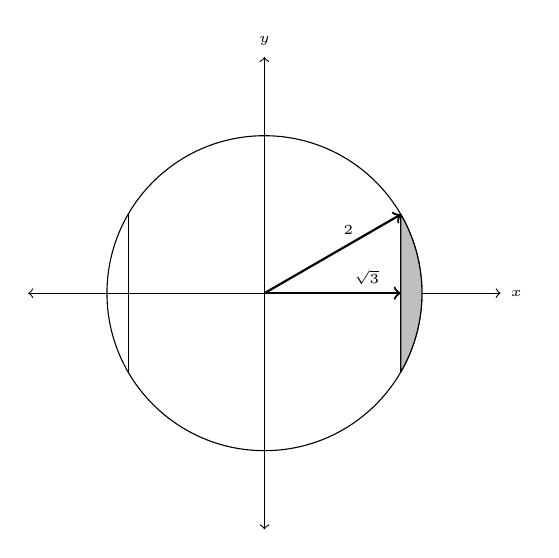
\begin{tikzpicture}
			\def \r{2}
			\def \rt{1.7321}
			\draw[->] (0,0) -- (3,0);
			\draw[->] (0,0) -- (0, 3);
			\draw[->] (0,0) -- (0, -3);
			\draw[->] (0,0) -- (-3,0);
			\draw[thick, ->] (0,0) -- (\rt,0);
			\node[] at (0.75*\rt, 0.2) {\tiny $\sqrt{3}$};

			\draw[thick, ->] (0,0) -- (\rt, 1);
			\node[] at (\rt/2+0.2, 0.5+0.3) {\tiny $2$};

			\node[] at (3.2, 0) {\tiny $x$};
			\node[] at (0, 3.2) {\tiny $y$};
			\draw[] (0, 0) circle (\r);
			\draw[] (\rt, 1) -- (\rt, -1);
			\draw[] (-\rt, 1) -- (-\rt, -1);

			\draw[fill=gray!50] plot[smooth, samples=100, domain=-1:1] %
			({sqrt(4 - (\x*\x))}, {\x}) -| (\rt, -1) -- cycle;
		\end{tikzpicture}
	\end{figure}
\end{frame}
\begin{frame}{10) continued}
	10. We can compute the volume of the portion cut out by finding the volume of revolution (about the $y-$axis) of the shaded part. This can be done easily using washer method.\\
	\[V' = \pi\int_{-1}^{1} \left(\sqrt{4 - y^2}\right)^2 - \left(\sqrt{3}\right)^2 dy = \frac{4\pi}{3}. \]
	The total volume of the ball is $V = \dfrac{4\pi}{3}(2)^2.$\\~\\
	Thus, the volume cut out is $V - V' = \dfrac{28\pi}{3}.$
\end{frame}
\end{document}

%---------------------------------------------------------

%Example of the \pause command
% \begin{frame}
%  in this slide \pause

% the text will be sounds partially visible \pause

% And finally everything will be there
% \end{frame}
%---------------------------------------------------------


% \section{Background of Shor's Algorithm}
% %---------------------------------------------------------
% \begin{frame}
% \frametitle{Background}
%     Let us look at the background of Shor's algorithm
%     \begin{itemize}
%       \item<1-> Quantum Algorithm, to find the prime factors of any given integer N
%       \item<2-> Named after a mathematician, Peter Shor who formulated the algorithm in 1994.
%       \item<3-> This algorithm cam factor a number N in $O((logN)^3)$ time and $O(logN)$ space.
%       \item<4-> This demonstrates that an integer factorization can be done on a quantum computer in polynomial time. 
%     \end{itemize}
% \end{frame}
% \begin{frame}
% \frametitle{RSA}
%     RSA is a popular encyrption technique that uses a public key N which is the product of two large prime numbers.
%     \begin{itemize}
%       \item<1-> One way to crack RSA encyrption is by factoring N, but, with classical algorithms, factoring becomes increasingly time-consuming as N grows larger.
%       \item<2-> More specifically, there is \textbf{no classical algorithm} known that can factor a number N in polynomial time.
%     \end{itemize}
%   \end{frame}
% \section{Grover's algorithm}

% \begin{frame}
%   Like many other quantum algorithms, Shor's algorithm is probabilistic. \pause
%   This means that it will give the correct answer with high probability, and the probability of success can be increased by performing more iterations.
% \end{frame}

% \begin{frame}
% Discrete Fourier Transform acts on a vector of complex numbers, $x_{0},x_{1},\dots , x_{N-1}$. of fixed length N, and outputs another vector of complex numbers,$y_{0},y_{1},\dots , y_{N-1}$ given by :
% $$y_{k} = \frac{1}{\sqrt{N}} \sum_{j=0}^{N-1}x_{j}e^{2 \pi ijk/N}$$ \pause
% The quantum Fourier Transform is defined in a similar way. The QFT on an orthonormal basis of vectors $\ket{0},\ket{1},\dots,\ket{N-1}$ is defined to be a linear operator with the following action on the basis state:
% $$\ket{j} \shortrightarrow  \frac{1}{\sqrt{N}} \sum_{j=0}^{N-1} \ket{k}e ^{2 \pi ijk/N}$$ \pause
% This can also be seen as :
% $$ \sum_{j=0}^{N-1} x_{j} \ket{j} = \sum_{k=0}^{N-1}y_{k} \ket{k}$$

% \end{frame}
%---------------------------------------------------------
% %Highlighting text
% \begin{frame}
% \frametitle{Introduction to Grover's algorithm}

% % In this slide, some important text will be
% % \alert{highlighted} because it's important.

% % Please, don't abuse it.

% % \begin{block}{Remark}
% % Sample text
% % \end{block}

% % \begin{alertblock}{Important theorem}
% % Sample text in red box
% % \end{alertblock}

% % \begin{examples}
% % Sample text in green box. The title of the block is ``Examples".
% % \end{examples}
% % \end{frame}

% Let us now look at another classical computing task that can be sped up using the superposition principle. \pause

% Our aim is to solve the needle in a haystack problem where we have to search for an element which satisfies a particular property, and it lies in a haystack of $N$ elements. \pause

% Classically, this would take $O(N)$ steps to do this task, but Grover's algorithm allows us to do it in $O(\sqrt{N})$ steps.
% \end{frame}

% \begin{frame}
%   \frametitle{Problem statement}
%   \begin{block}{Problem}
%     Suppose f(x) is a function from $\{0,1,\dots\}$ to $\{0,1\}$. f(a) = 1, only for one value of a. Find a. Assume that $N = 2^{n}$. This way you can work with n qubits.
%   \end{block}  
% \end{frame}

% \begin{frame}
%   \frametitle{Solution - Grover's Method}
%   \begin{center}
%     Let us define two new state vectors : \pause 
%   \end{center}
%   $$ \ket{\Psi_{0}} = \sum_{i=0}^{N-1} \frac{\ket{i}}{\sqrt{N}} $$ \pause
%   $$ \ket{e} = \sum_{i=0, i \neq a}^{N-1} \frac{\ket{i}}{\sqrt{N-1}} $$ \pause 

%   \begin{center}
%     Our goal is to ensure that we obtain $\ket{a}$ in the end. Notice that \pause
%     $$     \ket{\Psi_{0}} = \frac{\sqrt{N-1}\ket{e}+ \ket{a}}{\sqrt{N}}    $$ 
%     Thus $\ket{\Psi_{0}}$ lies in the subspace spanned by $\ket{e}$ and $\ket{a}$
%   \end{center}

% \end{frame}
% \begin{frame}
%   Note that, $\ket{\Psi_{0}}$ will be closer to $\ket{e}$ than $\ket{a}$. \pause
% %   \begin{figure}[htp]
% %     \centering
% %     \includegraphics[scale = 0.5]{grover.png}
% %   \end{figure}
% \end{frame}
% %---------------------------------------------------------
% \begin{frame}
%   We aim to take a vector $\ket{\Psi}$ which will initially be equal to $\ket{\Psi_{0}}$. \pause


%   Rotate it so that it ends up getting close to $\ket{a}$ \pause


%   First reflect $\Psi$ about $\ket{e}$ and then about $\ket{\Psi_{0}}$.
%   Reflecting about $\ket{e}$ can be considered as an oracle that performs the operation O
%   $$ \ket{x} \shortrightarrow (-1)^{f(x)}\ket{x}$$ \pause
%   The way to achieve this is to take an oracle that performs the operation 
%   $$ \ket{x}\ket{y} \shortrightarrow \ket{x} \ket{y \oplus f(x)}$$
%   Let $\ket{y}$ = $\frac{\ket{0}-\ket{1}}{\sqrt{2}}$ \pause
%   If x = a, $$\ket{x} \ket{y} \shortrightarrow - \ket{x} \ket{y} $$
%   Else, state will be preserved.

% \end{frame}

% \begin{frame}
%   \begin{block}{Remark}
%     It turns out mathematically, that Grover's operator G is 
%   $$G = (2\ket{\Psi_{0}}\bra{\Psi_{0}}- I)O$$ 
%   \end{block}
%   \pause 
% %   \begin{figure}[htp]
% %     \centering 
% %     \includegraphics[scale = 0.3]{Screenshot from 2021-07-19 22-30-03.png}
% %   \end{figure} \pause
%   Let $\ket{\Psi_{0}}$ make an angle $\theta$ with $\ket{e}$ in the two dimension subspace. Then,
%   $$ sin(\theta) = \frac{1}{\sqrt{N}} $$
% \end{frame}  
% %---------------------------------------------------------
% %Two columns
% \begin{frame}

% \begin{block}{Remark}
%   By induction, 
%   $$G^{k} \ket{\Psi_{0}} = cos((2k+1)\theta)\ket{e} + sin((2k+1)\theta)\ket{a}$$
% \end{block}
%  \pause 
% Applying G successively on $\ket{\Psi_{0}}$ rotates the vector by an angle $2\theta$ \pause 


% Goal is to make the angle between $\ket{\Psi}$ and $\ket{a} \le \theta$ \pause 


% Probability of collapsing will be $\ge cos(\theta) = \frac{\sqrt{N-1}}{\sqrt{N}}$ 

% \end{frame}
% \begin{frame}
%   \frametitle{Conclusion}
%   How many operations of G do we need though? \pause 
%   Clearly we require [$\frac{\pi}{4\theta}$] applications of G. As $\theta \ge sin(\theta) = \frac{1}{\sqrt{N}}$,
%   $$[\frac{\pi}{4\theta}] \le \frac{\pi \sqrt{N}}{4}$$ \pause 
%   Thus we need only $O(\sqrt{N})$ operations to achieve the task with probability $\ge \frac{\sqrt{N-1}}{\sqrt{N}} $

% \end{frame}
%---------------------------------------------------------


\end{document}s